La planificación de este Trabajo Fin de Máster se ha diseñado para que corresponda con el calendario de entregas propuesto por la Universidad Oberta de Catalunya.

En la gráfica de Gantt \ref{figure:gantt} se expone calendario iniciales de las actividades a planeadas al comienzo de esta investigación. Con color azul se han marcado las actividades relacionadas con la investigación y el estudio teórico, las tareas relacionadas con la implementación y cuestiones técnicas en color rosado y las actividades documentales y de divulgación en amarillo.

Respecto a la planificación inicial sólo se han eliminado la tarea de ``Bagging, boosting and stacking''. El tiempo asignado a éste se se ha redistribuido entre las tareas ``Optimización de los datos'' y ``Aplicación de Modelos''. En la imagen \ref{figure:ganttmod} se muestra gráficamente cómo fueron reorganizadas las tareas.

\begin{figure}[ht]
\centering
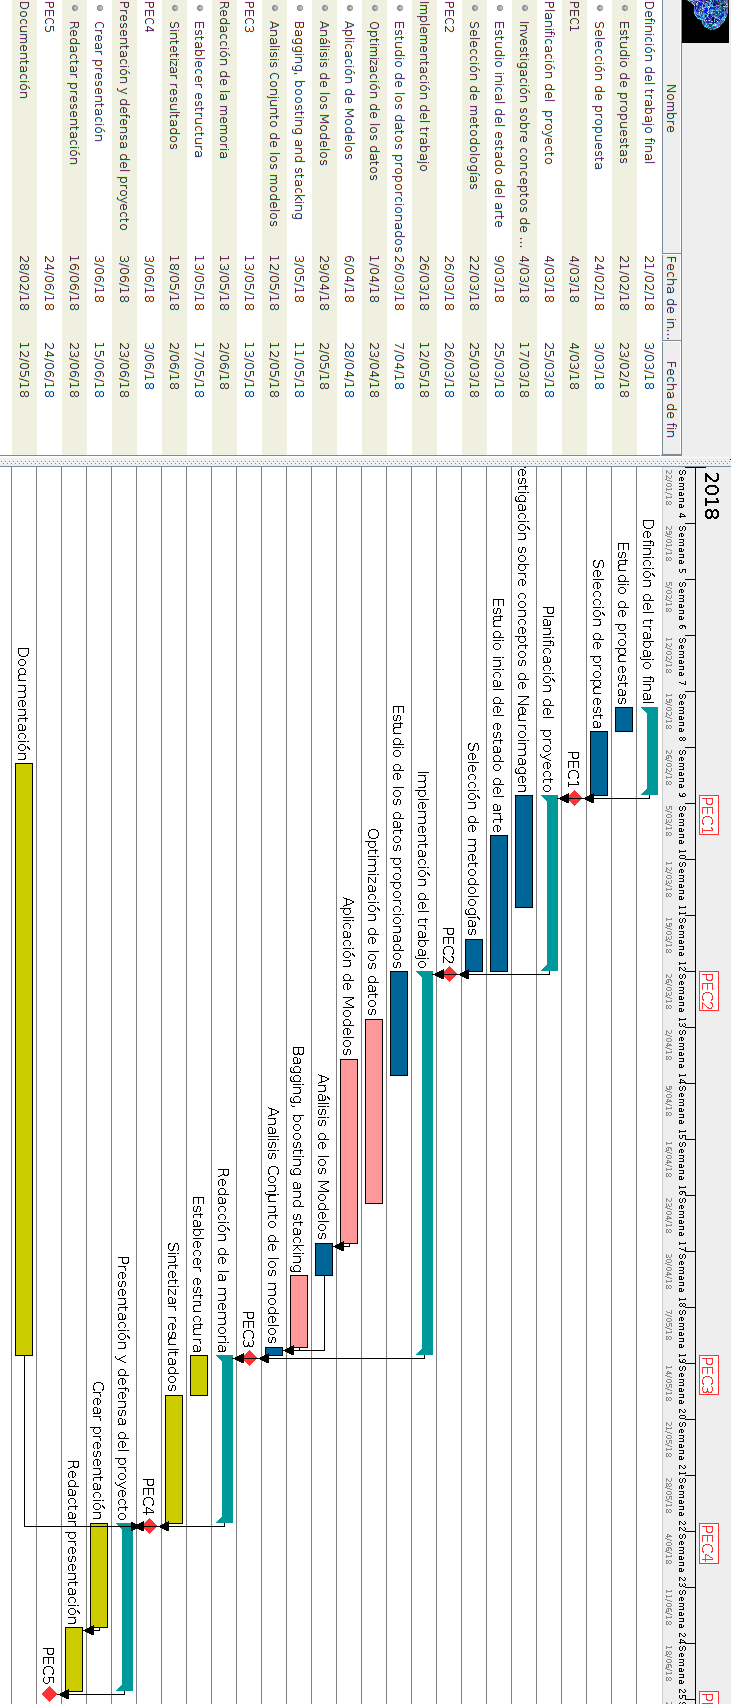
\includegraphics[width=0.6\textwidth]{figs/planificacion/gantt.png}
\caption{Planificación inicial en esquema de Gantt}
\label{figure:gantt}
\end{figure}

\begin{figure}[H]
\centering
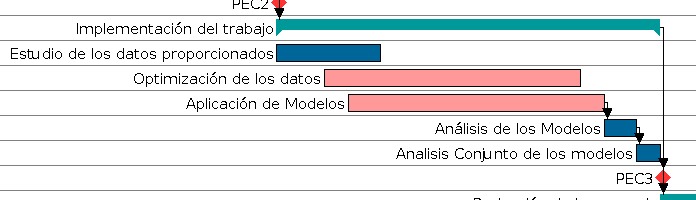
\includegraphics[width=0.6\textwidth]{figs/planificacion/modificacion.png}
\caption{Modificación en esquema de Gantt}
\label{figure:ganttmod}
\end{figure}